Um Informationen bzw. Bits zu manipulieren werden Schaltungen ben\"otigt welche Gatter beinhalten, dies gilt f\"ur klassische Rechner und Quantencomputer. Um in der Digitaltechnik die Funktionsweise von Gattern darzustellen werden gerne Wahrheitstabellen genutzt \ref{}. Bekannte Gatter-Typen aus der Digitaltechnik, wie der Negation oder dem Exklusiv-ODER k\"onnen auch in der Welt der Quantencomputer abgebildet werden. Jedoch ist der Aufbau dieser Gatter etwas gew\"ohnungsbed\"urfdig, denn die Realisierung dieser Gatter erfolgt durch unit\"are Matrizen. Die Anwendung eines Gatters auf einen Zustandvektor entspricht mathematisch also einer unit\"are Transformation auf den Zustandsvektor und f\"uhrt eine rotation auf der Bloch-Kugel aus. Dies geschieht durch die Bildung des Skalarprodukts \"uber der unit\"aren Matrix und dem Zustandvektor \ref{}. \\ \\
Eine Matrix wird als unit\"ar bezeichnet, wenn das Produkt aus dieser Matrix und dessen adjungierte Matrix eine Einhaltsmatrix bildet.
\begin{equation}
  I = A^{\dagger} A
\end{equation}
Die Adjungierte Matrix wird gebildet, indem alle Eintr\"age in dieser Matrix komplex konjungiert und transponiert werden.
\begin{equation}
  A^{\dagger} = A^{*T}
\end{equation}
Somit sind alle Quantengatter unit\"are Matrizen, genau wie die drei aus der Quantenmechnik bekannten Paulimatrizen $X, Y, Z$ \ref{tab:Qubit-Gatter}.

%%%%%%%%%%%%%%%%%%%%%%%Table%%%%%%%%%%%%%%%%%%%%%%%%%%%%%%%%

\begin{table}[h] \label{tab:Qubit-Gatter}
\begin{tabular}{@{\hspace{1cm}}c@{\hspace{1cm}} | @{\hspace{1cm}}c@{\hspace{1cm}} | @{\hspace{1cm}}c@{\hspace{1cm}}}
\hline 
Matrix & Schaltungssymbol & Wahrheitstabelle \\
\hline & \\
$X = \begin{bmatrix} 0 & 1 \\ 1 & 0 \end{bmatrix}$ &
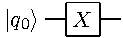
\includegraphics[width=0.2\textwidth]{figures/pauli_x.pdf} &
\begin{tabular}{|c||c||c|}
\hline
Fall & $|q\rangle$ & $X|q\rangle$ \\
\hline \hline 
1 & $|0\rangle$ & $|1\rangle$ \\
2 & $|1\rangle$ & $|0\rangle$ \\
\hline
\end{tabular} \\&\\

%%%%%%%%%%%%%%%%%%%%%%%%%%%%%%%%%%%%%%%%%%%%%%%%%%%%%%%%%%%%%%

$Y = \begin{bmatrix} 0 & -i \\ i & 0 \end{bmatrix}$ &
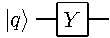
\includegraphics[width=0.2\textwidth]{figures/pauli_y.pdf} &
\begin{tabular}{|c||c||c|}
\hline
Fall & $|q\rangle$ & $Y|q\rangle$ \\
\hline \hline 
1 & $|0\rangle$ & $i|1\rangle$ \\
2 & $|1\rangle$ & $-i|0\rangle$ \\
\hline
\end{tabular} \\&\\

%%%%%%%%%%%%%%%%%%%%%%%%%%%%%%%%%%%%%%%%%%%%%%%%%%%%%%%%%%%%%%

$Z = \begin{bmatrix} 1 & 0 \\ 0 & -1 \end{bmatrix}$ &
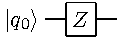
\includegraphics[width=0.2\textwidth]{figures/pauli_z.pdf} &
\begin{tabular}{|c||c||c|}
\hline
Fall & $|q\rangle$ & $Z|q\rangle$ \\
\hline \hline 
1 & $|0\rangle$ & $|0\rangle$ \\
2 & $|1\rangle$ & $-|1\rangle$ \\
\hline
\end{tabular} \\&\\

%%%%%%%%%%%%%%%%%%%%%%%%%%%%%%%%%%%%%%%%%%%%%%%%%%%%%%%%%%%%%%

$H = \frac{1}{\sqrt{2}} \begin{bmatrix} 1 & 1 \\ 1 & -1 \end{bmatrix}$ &
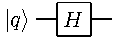
\includegraphics[width=0.2\textwidth]{figures/hadamard.pdf} &
\begin{tabular}{|c||c||c|}
\hline
Fall & $|q\rangle$ & $H|q\rangle$ \\
\hline \hline 
1 & $|0\rangle$ & $\frac{|0\rangle+|0\rangle}{\sqrt{2}}$ \\
2 & $|1\rangle$ & $\frac{|0\rangle-|1\rangle}{\sqrt{2}}$ \\
\hline
\end{tabular} \\&\\

%%%%%%%%%%%%%%%%%%%%%%%%%%%%%%%%%%%%%%%%%%%%%%%%%%%%%%%%%%%%%%

$S = \begin{bmatrix} 1 & 0 \\ 0 & i \end{bmatrix}$ &
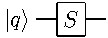
\includegraphics[width=0.2\textwidth]{figures/phase.pdf} &
\begin{tabular}{|c||c||c|}
\hline
Fall & $|q\rangle$ & $S|q\rangle$ \\
\hline \hline 
1 & $|0\rangle$ & $|0\rangle$ \\
2 & $|1\rangle$ & $i|1\rangle$ \\
\hline
\end{tabular} \\&\\

%%%%%%%%%%%%%%%%%%%%%%%%%%%%%%%%%%%%%%%%%%%%%%%%%%%%%%%%%%%%%%

$T = \begin{bmatrix} 1 & 0 \\ 0 & e^{i\frac{\pi}{4}} \end{bmatrix}$ &
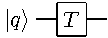
\includegraphics[width=0.2\textwidth]{figures/t_dagger.pdf} &
\begin{tabular}{|c||c||c|}
\hline
Fall & $|q\rangle$ & $T|q\rangle$ \\
\hline \hline 
1 & $|0\rangle$ & $|0\rangle$ \\
2 & $|1\rangle$ & $e^{i\frac{\pi}{4}} |1\rangle$ \\
\hline
\end{tabular} \\&\\
\hline
\end{tabular}
\caption{Grundlegende 1-Qubit Gatter}
\end{table}
